% !tex root = ../Thesis.tex

\section{Problem Statement}

\color{red}
To Do:
\begin{itemize}
	\item Describe what pitch correction is
	\item Describe why it is difficult
	\begin{itemize}
		\item Pitch detection is not trivial
		\item Why you can't just speed up sound and slow it down
		\item Convey the essence of the problem
	\end{itemize}
		\item Motivate why it's needed
		\begin{itemize}
		\item One small out of tune note causes a whole new re-recording
		\item Quick fix after recording
		\item Live performers can now sing
		\item Produces a quirky robotic effect that can be desirable
		\item Case against audio pitch correction
		\begin{itemize}
			\item Less freedom to professional singers
			\item Vibrato, colour etc
			\item Conceals talent
		\end{itemize}
		\item Biggest case for: Interesting mathematical project
	\end{itemize}
\end{itemize}
\color{black}

\section{History of Audio Pitch Correction}

One of the first occurrences of pitch manipulation in music, at least the first
occurrence that was found by the author, was of a song called ``The Chipmunk
Song'' from the animated music group ``Alvin and the Chipmunks''. The goal was to
raise the pitch of the voice of a singer to sound an octave higher than his actual
voice. This was accomplished by recording the song at half the wanted tempo and
playing back the recording at twice the speed when mixing. The technology used in
audio recordings was still analog tape recordings and the whole process was done
using these tapes. The effect of speeding up a recording to achieve a pitch
shift became known as the ``Chipmunk Effect''. The approach earned the group two
Grammy awards in 1958.

In 1977 Eventide introduced a new product, the Eventide H949 Harmonizer, capable
of incremental pitch shifting. This was sold as a ``de-glitch pitch shifter'' and
was intended to be used to fix intonation errors and add harmonization effects
after recording. Other features commonly used was to stretch the time of radio
recordings of advertisements to be an exact duration without affecting the pitch.
The pitch shifting was implemented using single side-band modulation
techniques and was done digitally.

\begin{figure}[h]
	\centering
	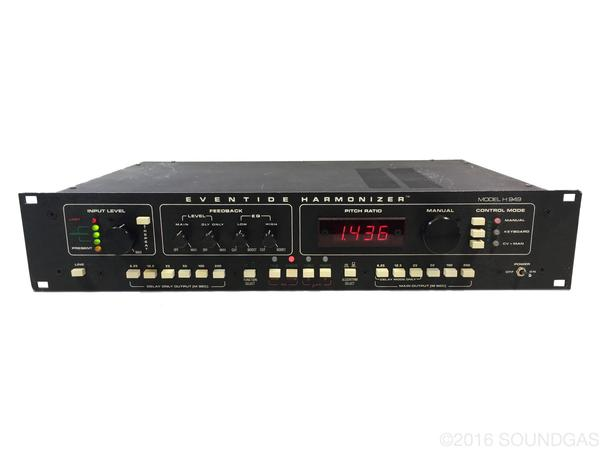
\includegraphics[width=0.9\textwidth,trim={0mm 55mm 0mm 55mm},clip]
	{EventideH949}
	\caption{Eventide H949 Harmonizer Rack Mounted Unit}
	\label{fig:EventideH949}
\end{figure}

In 1996 Andy Hildebrand, an electrical engineer, was investigating seismic data
when he realised that the same techniques he was using to investigate the data
could be used to alter the pitch of audio files. His techniques for detecting
pitch, using a simplification of the autocorrelation function, was considered
superior to the state of the art at that time. He implemented the first version of
his pitch correcting algorithm on his Macintosh computer. His first demonstration
was considered a success and the company ``Antares Audio'' was founded. They
created a product called ``AutoTune'' which was popularised in 1998 by Cher in her
song ``Believe''.

\begin{figure}[h]
	\centering
	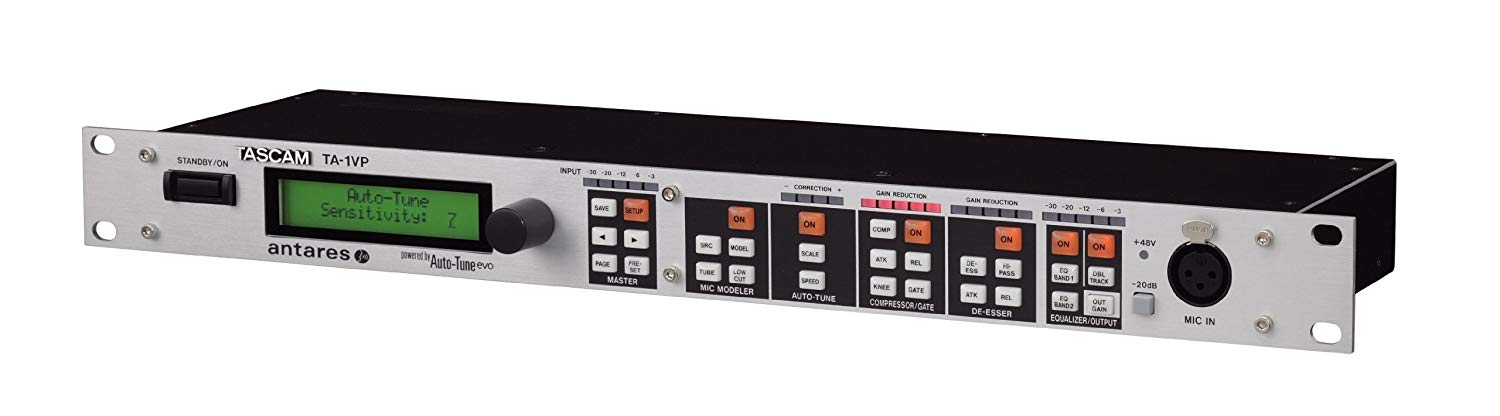
\includegraphics[width=0.9\textwidth,trim={30mm 20mm 30mm 30mm},clip]
	{AutoTuneRack}
	\caption{AutoTune Rack Mounted Unit}
	\label{fig:AutoTuneRack}
\end{figure}

AutoTune comes in a rack mounted unit for live performances shown in figure
\ref{fig:AutoTuneRack} or as a plugin with the interface shown in figure
\ref{fig:AutoTunePlugin}. The software has evolved to allow for many more features
than the original pitch correction effect that the name suggests. Modern AutoTune
is still considered the state of the art product by audio engineers.

\color{red}
To Do:
\begin{itemize}
	\item Open source pitch correction AutoTalent by Tom Baran
	\item Smule App
\end{itemize}
\color{black}

\section{Approach Taken}

\color{red}
To Do:
\begin{itemize}
	\item Discuss structure of report
	\item Show final implementation
	\item Summarise results and conclusion section
\end{itemize}
\color{black}
